\emph{The Monitor Celestra} is a game that transformed a World War II era battleship into a space ship, inviting the participants of the game to enter the Battlestar Galactica\cite{larson_battlestar_1978} universe and forge their own path into the future. The game, a Nordic Style Live Action Roleplaying Game (LARP) assigns roles to the participants -- as crew, passengers and refugees on board the space ship -- and act out the resulting story within a framework of plots, story lines and clues. The medium differs from theatre plays in the lack of a script and from improvised theatre in the lack of an audience -- to consume the medium is to participate in it.

Nordic Style LARPs are characterized, among other things, by a strong focus on immersion. The goal is for participants to feel embedded in the game world without the distraction of the real world disturbing the fiction. In recent years, more and more games have been organized that include technological support to improve the feeling of immersion into the game world.

For \emph{The Monitor Celestra}, full immersion was implemented using a number of different techniques: the signage of the ship was replaced with signs that were
in the Battlestar Galactica aesthetic, the ship
had custom-built control panels controlled a space dynamics simulator, and the game
master team had the ability to trigger a large array of scripted, partially scripted or improvised events that launch sounds and influence the ship control panels to convey the story.

An important part of this immersion was 15 pairs of
loudspeakers, each pair hooked up to a Raspberry Pi\cite{rpi} and
connected to a wired ethernet network. These loudspeakers played
localized sound effects as well as an ambient sound backdrop through
the entire game, drowning out the sounds of inner city Gothenburg and
supporting the game experience by confirming consequences of player
actions through mediated responses.

\section{Background}
\label{sec:background}

LARP is a form of game where participants receive roles and then proceed to enact their roles within a framework of plots, story lines and clues. Traditionally, LARPs have been focused on telling stories in a fantasy/medieval setting, but the form has seen a wider spread of genres over years. LARP has developed into various design schools and style -- mostly based on geographical distribution. Thus, there are Nordic LARPs, American LARPs and Russian LARPs, to name a few\cite{kp2011}. Each school of design has its own theories on what constitutes a good LARP and what goals one must strive to achieve with the game design, participation and outcome of the game.

In the same tradition as table-top role playing games and improvisation theatre, LARP is played out by players in real time in the same general physical area. Players wear costumes and make props to better simulate their respective characters. In general, participants receive instructions beforehand regarding specific game rules, other characters, shared background information, etc. Organizers define social mechanics and hard game rules for resolving combat, conflicts or sex. 

\subsection{Nordic LARP}

\emph{The Monitor Celestra} belonged to the Nordic LARP school of design. This school could be argued to emphasize a few different points as being major when creating or participating in the experience: 

\begin{itemize}
    \item The game should represent the world as faithfully and completely as possible (games which fulfill this criterion are commonly referred to as 360\degree{} games.) Everything players see and/or experience represents itself within the game -- a gun is a gun, a knife is a knife.
\item Participants should put emotional engagement and experience above achieving in-game goals. Powerful emotional impacts should take precedence when deciding how to move the game forward.
\item The players should control the outcome of the game. While parts of the game might be scripted, the main outcome of the game should be left to the players as far as possible.
\end{itemize}

Due to the nature of the Nordic school of design, games designed within that school tend to focus on moral choices and complex social interactions rather than traditional fantasy stories. There have been games depicting everything from Danish hobos on the road (\emph{The White Road}~\cite{pedersen2008}) and students investigating possessed ladies (\emph{Prosopopeia}~\cite{jonsson2006prosopopeia, montola2006prosopopeia}), to 1950s families hiding from nuclear war (\emph{Ground Zero}~\cite{nordiclarp}) and terminal cancer patients (\emph{Luminescence}~\cite{nordiclarp}).

\subsection{LARP vs. Similar activities}

What separates LARP from other similar activities such as tabletop
roleplaying games, computer games and improvised theatre is still an
open question. Researchers~\cite{montola2012,turku3,henriksen2004}
have pointed to a few main points; 

\begin{itemize}
\item Emotional engagements increased radically when players are physically engaged in the activity~\cite{turku3}.
\item Moral choices and consequences from player actions have larger impact when acted out by other physical players~\cite{turku3}.
\item Players allow themselves more freedom when acting within a ludic circle,\musthavefootnote{\textit{ludic circle}: a shared space of playfulness, from \textit{ludic}: playful} thus allowing for a wider range of emotions, experiences and shared actions~\cite{montola2012,stenros2012}.
\item Reflections on the complexity of social and/or humanistic behavior or models yield a higher level of understanding~\cite{henriksen2004}. Research has shown that when trying to understand complex models of human behaviour, both in extreme situations such as emergencies and in everyday contexts - LARP tend to work very well as tool for exploring motivations, social roles and social systems based on incitements
\end{itemize}

It has been humorously suggested that LARPing may be seen as the ``extreme'' sport of interactive experiences due to the efforts involved with staging and participating in games, the impact on participants and the cumulative effects of player actions and organizer design.

\subsection{Similar Events}

There have been other efforts to use technology to enhance LARP experiences within the game\musthavefootnote{As apart from using techonology for support functions, such as economy, participant management etc.} as a key part of staging the experience, mainly within the Nordic school of LARP design. Historically, these experiments have been conducted by a small number of game designers and writers. Experiences where technology were used in a similar capacity as on \emph{The Monitor Celestra} includes: 

\begin{itemize}
\item \textbf{Prosopopeia: Bardo 1} A technology-enhanced LARP played in the autumn of 2005. Players used technology concealed in an old reel-recorder to communicate with dead spirits.
\item \textbf{Prosopopeia: Momentum} An continuation to the Prosopopeia project, \emph{Momentum} played in the autumn of 2006. Players used a wide variety of technology, including hardware built using custom constructed components to explore and wage battles against forces on the other side of death. 
\item \textbf{Felsäkert Läge} A technology-enhanced LARP in the autumn of 2010 situated in a future, post-apocalyptic world, staged in an abandoned mining town in the north of Sweden. Technology was used to simulated surviving technology from before the catastrophe, telling stories and providing quests, items and treasures for the players to find and use in their own game.
\end{itemize}

An overview of similar experiments (and others) can by found in~\cite{nordiclarp}.

\subsection{Immersive Soundscapes}
Earlier efforts on immersive soundscapes include various implementations in Python, support in most holistic game engines and similar. However, the main difference between these implementations and the system built for \emph{The Monitor Celestra} is the spatial scale. Usually, these soundscapes are meant to be enjoyed by a single person in headphones or a handful of persons in a single or a few rooms. 

The difference in scale between these implementations and the one described in this paper makes comparisons hard to do. Most issues met by the usual implementations were either deemed irrelevant (such as super-focused spatial placement in the scene -- a rough idea was more than enough for a battleship) or too specific (solutions for physical placing loudspeakers in a square room). 

\begin{figure}[H]
  \centering
  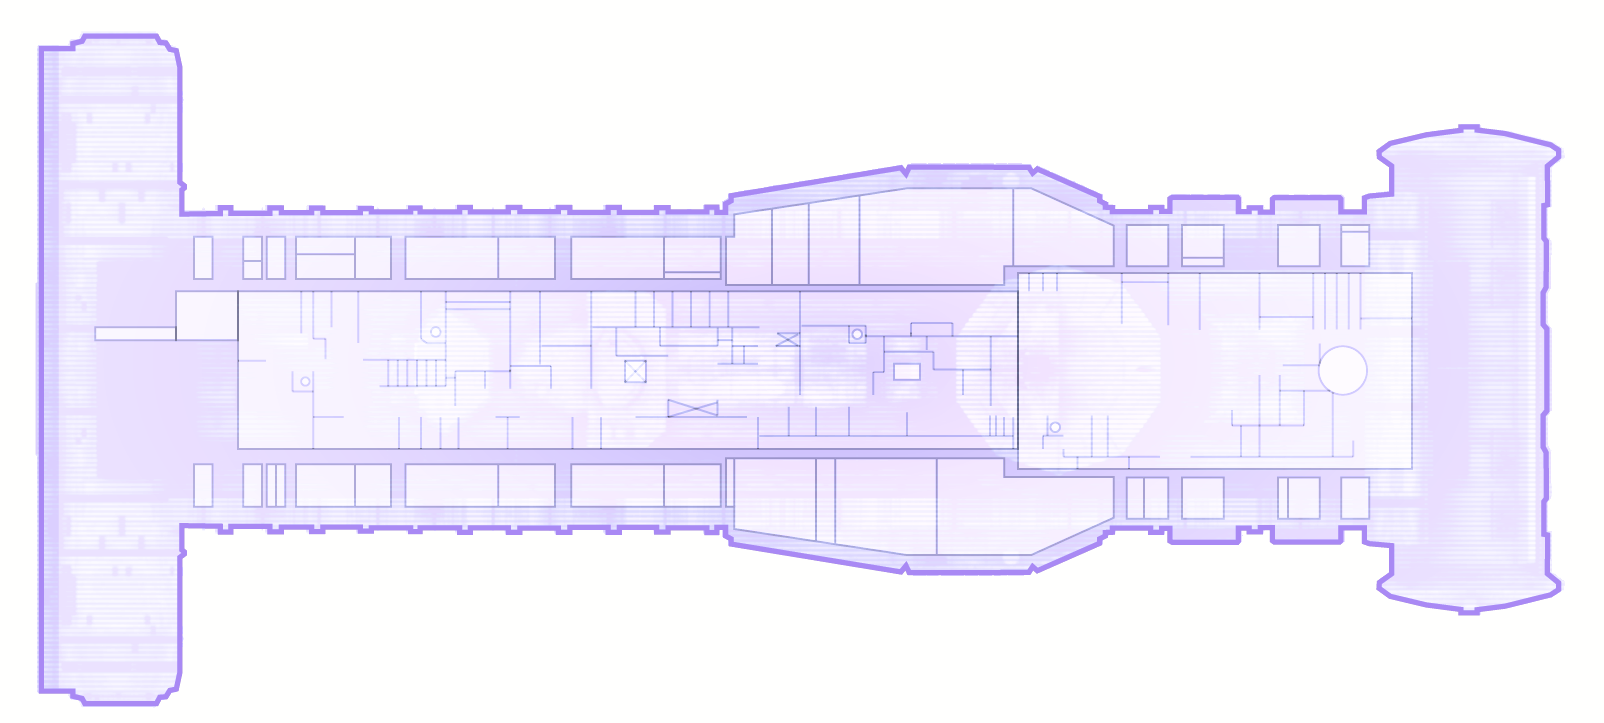
\includegraphics[width=0.6\textwidth]{img/ship}
  \caption{Floor plan of The Monitor Celestra}
  \label{fig:celestra}
\end{figure}

\subsection{Structure of The Monitor Celestra}
Every LARP differs in structure and design according to the design goals, creators and aims with the project. The Monitor Celestra had three runs with 150 participants each, split over three weekends. The runs were separated from each other and played out the same story with different participants (even though some participants bought tickets for all the runs). 

Every run was split into four game sessions of 4--6 hours, with breaks between for sleep and briefings. Food was distributed and eaten while in play. Even though the battleship Småland was equipped with bunks for its crew, fire regulations prohibited sleeping on board the ship. Hence, the participants slept at a nearby hostel between game days.

The story design started out in the setting of Battlestar Galactica: a fleet of refugee spaceships carrying most of the remainder of humanity flee from robot aggressors. In the game, The Celestra is separated from the remaining fleet by accident, and the players have to decide on their actions, while facing various threats: robots hunting them down, colonies with radical political views and demands, and internal conflicts on board the ship. Each of the games ended in a different way, ranging from a valiant effort to save the human race by nuclear suicide taking out a threat before it could reach the rest of the fleet to setting course for deep space and forging a new path for the isolated ship.



%%% Local Variables: 
%%% mode: latex
%%% TeX-engine: default
%%% TeX-master: "tmr"
%%% End: 
